%%%
% Tech report template. Compile with pdflatex
%%%
%\documentclass[pdftext,twoside,10pt]{report}
\documentclass[pdftext,twoside,10pt]{article}

\usepackage[a4paper,lmargin=2cm,rmargin=2cm,tmargin=.7cm,bmargin=1cm,includehead,includefoot]{geometry}
\usepackage[german,english]{babel}

\usepackage{subfig}
\usepackage[small,compact]{titlesec}  %for compressed Section titles
\usepackage{times}
\usepackage[T1]{fontenc}
\usepackage[utf8]{inputenc}
\usepackage{graphicx} 
\usepackage{pgf}
\usepackage{hypernat}
\usepackage{hyperref}
\usepackage{multicol}
\usepackage{wrapfig}
\usepackage{multirow}
\usepackage{comment}
\usepackage{rotating}
%%% Package options %%%
\makeatletter
\newenvironment{tablehere}
  {\def\@captype{table}}
  {}
\newenvironment{figurehere}
  {\def\@captype{figure}}
  {}  
\makeatother
\hypersetup{colorlinks=true, breaklinks=true, pagebackref=true,
  urlcolor=blue, linkcolor=blue,anchorcolor=blue,citecolor=blue,
  pdfpagemode = UseNone, %FullScreen, %UseThumbs, %UseOutlines,
  pdfauthor = {},
  pdftitle = {},   
  pdfsubject = {},
  pdfkeywords = {}
}
\DeclareGraphicsExtensions{.jpg,.pdf,.mps,.png}


\usepackage{xcolor}

\setlength{\parindent}{0cm}

\urlstyle{rm} %so it doesn't use a typewriter font for urls.
\renewcommand{\captionfont}{\small \sffamily}
\renewcommand\floatpagefraction{.9}
\renewcommand\topfraction{.9}
\renewcommand\bottomfraction{.9}
\renewcommand\textfraction{.1}   


\definecolor{blue}{RGB}{30,30,150}
\newcommand{\spag}{\textcolor{red}{SPAGHETTI CAT!!}}
%  Title page
\title{CollideFx}
\author{Chet Gnegy}

\begin{document}

\maketitle

\section{Introduction}
The purpose of this project is to create a real-time audio effects processor with a graphical interface that integrates the physics of real objects as well as the actions of the user into the parameter space of the signal chain. The basic design is as follows: There are a bunch of different modules that can be placed in a 2D plane, each of these modules has physical properties assigned to it and can impact the sound of some input source. The modules are represented by short cylinders, called Discs. The Discs are each associated with some unit generator, whether it be an input source or an audio effect. The proximity of the Discs to one another will determine the signal path as well as the mix level for the effects. The user, who can interact with the environment through clicking, can drag the Discs around the world, changing signal flow graph. The Discs are bound to the laws of physics, however, and will bounce off of one another as well as with the walls of the environment. The physics engine is also responsible for computing friction and angular velocities, the latter of which could also be mapped to a parameter of the unit generators in future iterations.


\begin{figure}[b!]
  \centering
    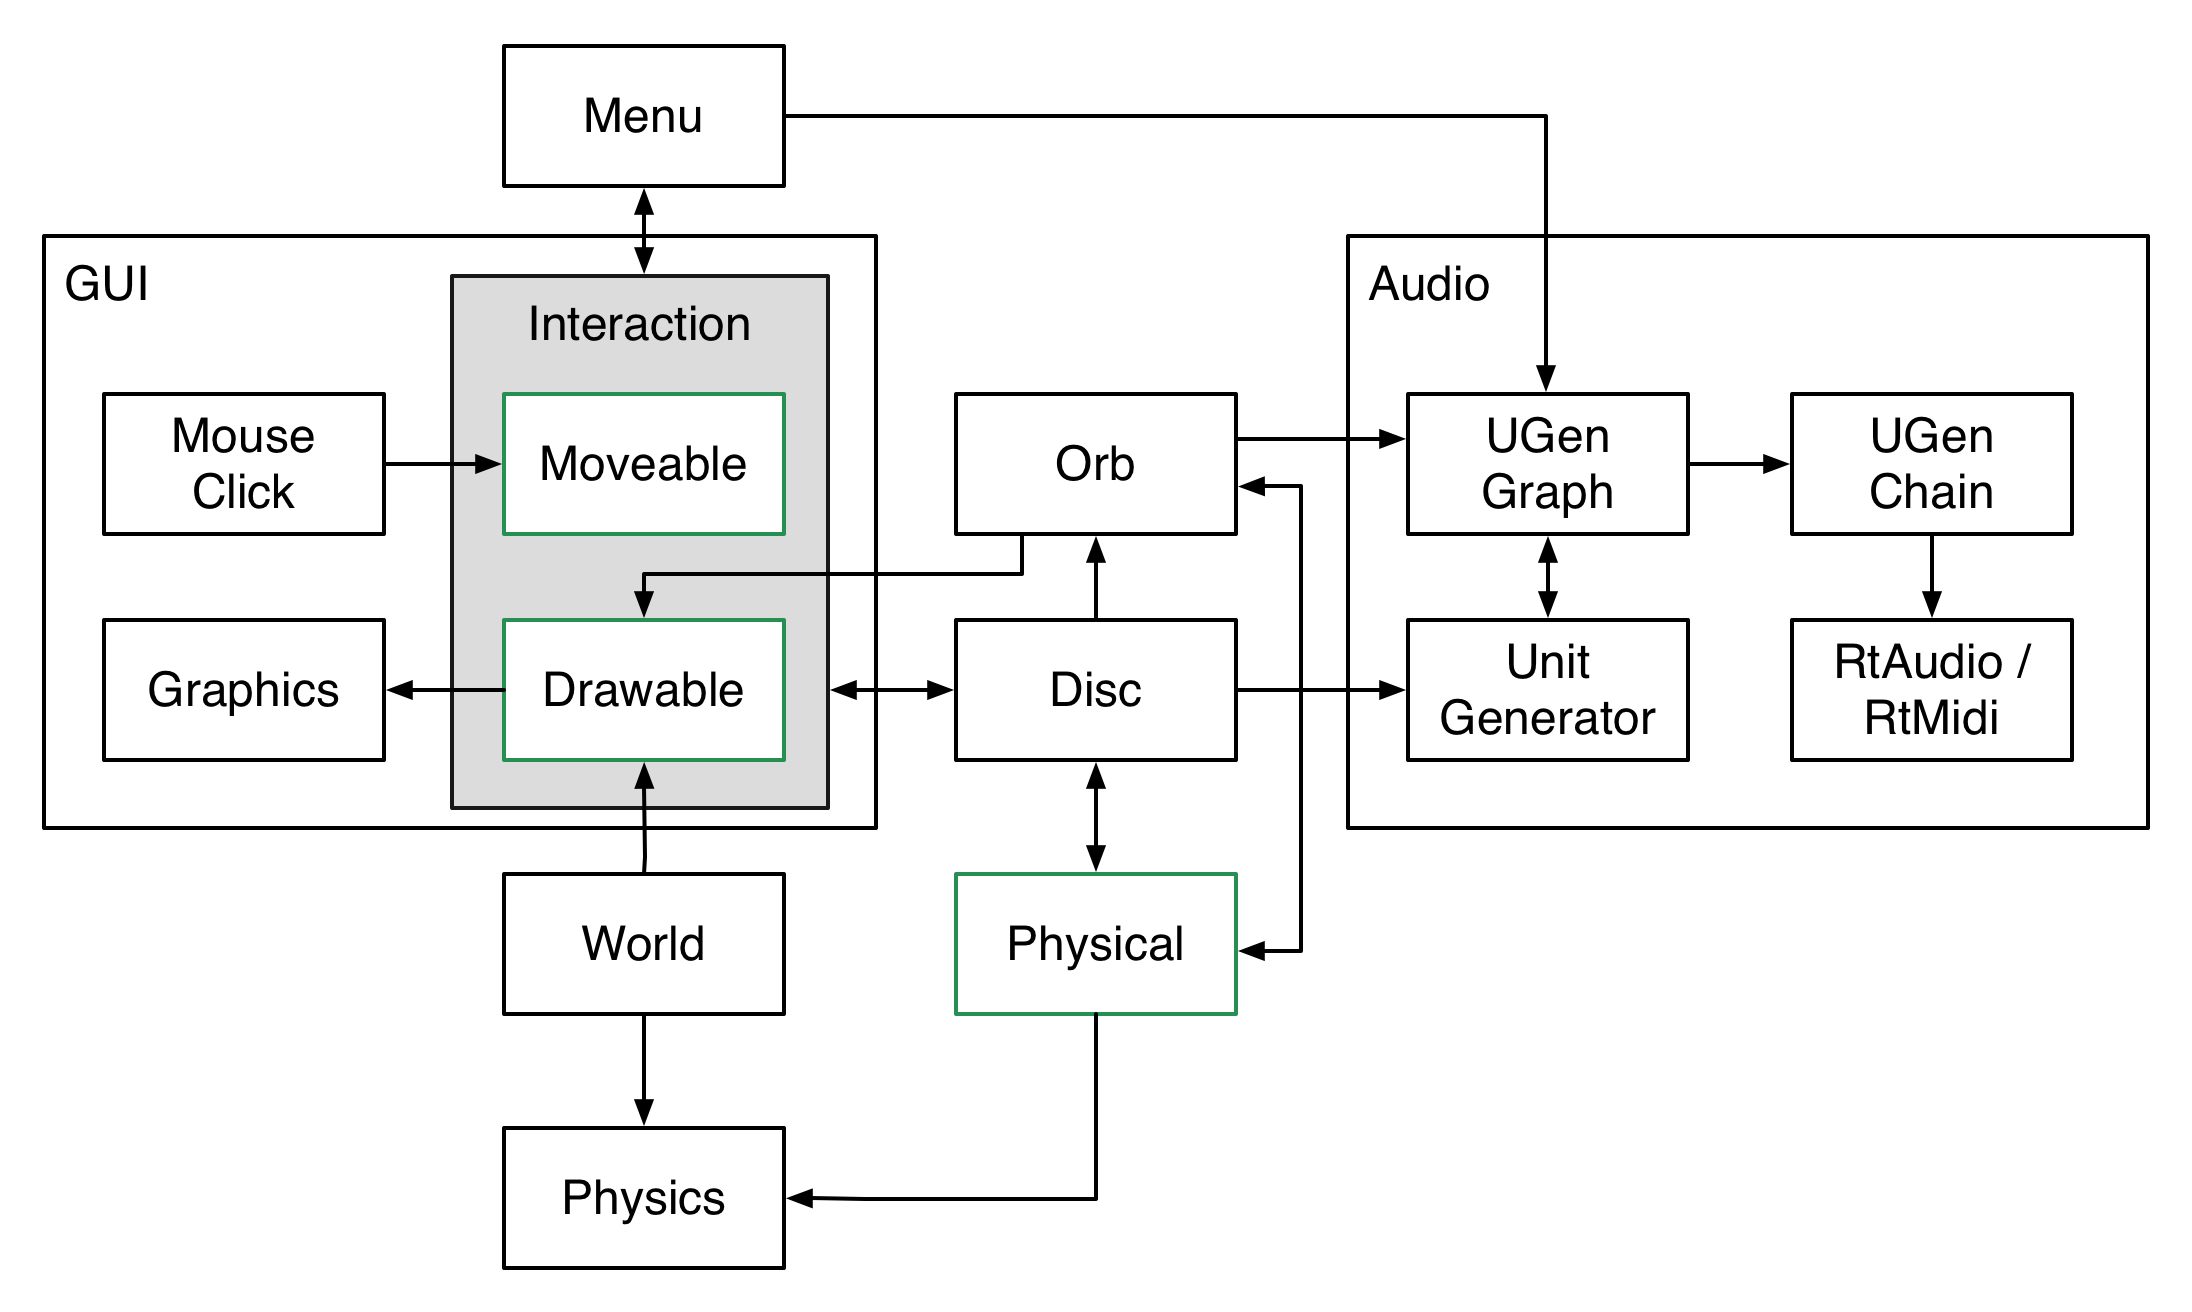
\includegraphics[width=\textwidth]{flow.png}
    \caption{The system diagram.}
  
\end{figure}


\section{Audio Framework}

This software utilizes the RtAudio$_{[1]}$ engine, which conveniently allows the system to communicate with the sound card by periodically filling buffers with audio data. To keep the system modular, the graphical display and the audio components are completely independent of each other and interact only through the parameter space of the Disc objects. The RtAudio callbacks are handled through by UGenChain class. UGenChain contains a graph of UnitGenerators that pass the audio signal from the input source to the next element in the chain and finally to the array designated as the output buffer. The graph is stored in the UGenGraphBuilder.

\subsection{Signal Path}
The UGenChain class has three main responsibilities: handling the audio stream, providing the next sample of audio data on request, and making sure that Midi information is delegated to the signal flow graph. The first of these responsibilities involves only initializing the RtAudio engine and opening the audio stream. The provision of the next sample is fairly straightforward given that the chain of unit generators. We simply "tick", or compute one sample, of audio from each unit generator in order and pass the result from the next. We of course start with an input source, who simply returns a sample of the audio input. Midi sources return a single frame of audio data based on the Midi information provided and the type of waveform. The effects units are similar but involve some calculation, often state-based depending on its parameters, and also on the samples that have been processed by it at previous times.\\

\subsection{Unit Generators}
Several unit generators have been defined for this software. Many of them are loosely based around well known DSP algorithms. The unit generators feature two main methods, "tick" and "set\_params". As previously mentioned, "tick" processes a single sample of audio data. The method "set\_params" allows for the parameters of the unit generator to be changed. This does not include the parameters that are determined by the position of the Discs, but some internal parameters to the unit generator. The UGenGraphBuilder and UGenChain classes provide the input data to the unit generators in the form of an audio buffer or a midi event. In the following section, we discuss the various types of unit generators.


\subsubsection*{Audio Input and Midi Unit Generators} The Input unit generator simply listens to the computer's designated input channel. In the absence of any other unit generators, the input is simply delivered back to the output. Additionally, we have several midi unit generators, all using classic waveform generators to provide audio data to the other modules. The audio and midi data is passed from a callback in the UGenChain to the UGenGraphBuilder and then to the individual audio and midi modules. Each midi module has an attack and sustain parameter allowing some configuration of the sound. The midi waveforms are all produced using additive synthesis. As many as 15 harmonics are used to generate the waves. This was done to reduce the harshness of the ideal square, saw, and triangle waves caused by discontinuities in amplitude or in their first derivative.

\subsubsection*{Bit Crusher}
The bit crusher effect is very handy for reproducing vintage low-fi audio effects. The audio signal, typical 16 bits in resolution, is quantized down to a specified level on the range of 1 to 16, 16 being the unquantized signal. By using a value of 8 bits, we can achieve "chip music" sounds that resemble those of older game systems. The bit crusher also features a downsampling parameter which effectively reduces the sampling rate of the signal. We can downsample by an integer number on the range 1 to 16, where we quickly experience the effects of aliasing as this parameter increases.

\subsubsection*{Chorus} 
The chorusing effect used is modeled as described in Jon Dattorro's paper on delay-line modulation$_{[2]}$. The effect is achieved by summing the dry signal, $x(t)$, with a delayed copy of itself, $x(t - \tau(t,f_c,d_c))$, where $\tau(t,f_c,d_c) =d_c$sin$(f_ct)$. The modulation rate, $f_c$ is bounded on the range 0.02 - 10.0 Hz, and the depth of the effect,$d$ is bounded by 0.0125. There is also a negative feedback path with a delay of $\tau(t,f_c,0)$, corresponding to the average delay length of the feedforward path. The weighting of each of these paths is given by Dattorro's "white chorus".

\subsubsection*{Delay}
This is a simple delay line. The time in seconds can be changed as well as the amount of feedback.

\subsubsection*{Distortion}
The distortion module is pretty simple, it limits the input using an arctangent function. The controllable parameters are the input and output gain.

\subsubsection*{Filters}
There is a choice of low and high pass both selectable using the Filter unit generators. The Filter ugen can be toggled between high and low pass. For all filters, the cutoff frequency and Q can be changed.

\subsubsection*{Granular}
The granular synthesis module holds a two second buffer of its most recent input. A given length of consecutive samples, a granule, is pulled from a random point in the last two seconds and multiplied by a raised cosine window. The samples are triggered randomly such that there are always roughly 10 samples playing at once. The user can change the length of the granules as well as the frequency at which they are triggered, a parameter called Density. Shorter granule lengths create noises that are less similar to the input.

\subsubsection*{Looper}
The looper waits for the user to trigger a start event and begins to count down from a designated number of beats. It then records its input for a given number of beats at a specified tempo. Immediately after completing the recording, it begins to replay the buffer on repeat. Effects can be applied to the looper as if it is an input. Once the looper has started a recording, its parameters are immutable, except for the count in. To record or re-record the into the looper, double click on it and begin playing once the count down has finished. Once the looper is in playback mode, the signal graph is recomputed, considering it to be an input.

\subsubsection*{Ring Modulator}
The ring modulator multiplies the input by a simple sinusoid. The frequency of which is chosen by the user.

\subsubsection*{Reverb}
This is an implementation of Freeverb$_{[3]}$ using feedback comb filters and all pass filters. The size of the simulated room and the damping can be altered in real time.

\subsubsection*{Tremolo} 
The tremolo module provides simple low frequency amplitude modulation with a sinusoidal carrier wave. The modulation rate, $f_t$ is bounded on the range 0.02 - 10.0 Hz.




\subsection{Graph-based Signal Flow}
Finally, the signal chain is determined. This is done by the UGenGraphBuilder class. The UGenGraphBuilder considers the locations of the Discs in the world and contsructs a Minimal Spanning Tree, where the Discs are treated as Nodes, and the connections between them as Edges. A modified version of Prim's Algorithm is used to construct the tree. This provides an intuitive looking graph, (i.e., the nodes closest to each other are connected). It also prevents the formation of cycles, which would cause the system to possibly be unstable. The algorithm is modified in three ways, the connections will not be made if the distance between two nodes exceeds some maximum distance. There is also a condition that prevents two input discs to be connected to each other. This includes the audio and midi inputs, but not the looper effect (discussed later), though it can provide input to the other generators. Because the nodes can be too far away, the tree may be completely disconnected, or in sections. Prim's algorithm does not deal with disjoint trees, so we include a final modification such that all nodes must be at least attempt to connect to the tree. The algorithm runs until all nodes are designate ``marked" either by connecting them to a tree or by running through the algorithm and finding that a connection cannot be made. These connections are recorded in objects called Wires.\\

The signal must be passed from source to the implicit sinks (a unit generator with no output), this implies that the directionality of the Wires is critical. We resolve the directionality of the network of wires iteratively. We start by ensuring that any nodes labeled as inputs are on the ``From" end of the wire. The discs on the ``To" end of these wires must naturally be the ``From" end of any wires leading out of those discs. We iteratively swap wires from the beginning to the ends of the chain to make sure that paths are leading away from inputs. Because the directionality may be sensitive to the order that it falls in the wire list, we first sort the wire list. The wire list is sorted using the addresses of the connected discs using the ``From" disc as a key, and the ``To" disc as a secondary key. The addresses are used because they will not change over the course of their lifetime and because they should be roughly independent of any properties of the disc.\\

Once the chain is computed, a data structure that holds the inputs and outputs of each disc is linked to the discs. Sinks are marked and pulled for output samples. We recursively ask the sink nodes for their outputs, which compute something based on their inputs. To get the inputs we ask the input connections for their output samples. Of course, the inputs need computed before the outputs, so, we use a tail recursive tick function to calculate this conveniently. This function scales down the signal amplitudes by a factor of $\frac{1}{\sqrt{k}}$, where $k$ is the fanout of the previous unit generator in the chain. This keeps the signal at roughly the same amplitude even when the signal branches out many times. The square root is used because loudness is proportional to the square of amplitude. The mix levels are also computed here. 


\section{Graphics}
The OpenGL library is used to provide a graphical interface for the project. The two main classes of displayable objects are the "World" and the "Disc". Each instance of these classes implements an interface Drawable, which allows for clean integration with the OpenGL module. OpenGL need only hold on to a list of Drawable objects, and the individual classes are responsible for their own rendering instructions. The drawable objects have an associated priority. High priority objects sit at the beginning of the list and are drawn first. The menu and the world have the highest priority, followed by the discs and the particles that float around them, called orbs. There is also an interface, Moveable, that allows the user to manually operate on the objects in the world using the mouse.

\subsection{The Drawable and Moveable Interfaces}
Drawable is an abstract class containing only pure virtual methods. The Graphics module holds on to a list of drawables, and each one is responsible for the actual display instructions. Similarly, the Moveable interface is responsible for how the objects interact with the click. Once an object is clicked, dragged, or unclicked, its clicked, move, or unclick methods are called. These interfaces keep the Graphics module neat and clean, allow for new objects to be easily drawn and integrated, and keep everything modular.

\subsection{World}
The world consists of a square shaped grid with wireframe boxes as walls. There is a glowing grid along the bottom of the world with orbs that randomly traverse from one side to the other. Both the grid and the orbs are implemented as textures. The grid and the orbs brighten and fade in sync with each other. The borders glow out of phase with the center of the grid to give the appearance that energy is being transferred from one to the other.

\subsection{Discs}
The discs are simple cylinders with orbs floating around them. The discs feature an image that details what the disc's purpose is. For example, the audio input disc has an audio waveform on it, and the delay disc has an image of a stop watch. The input discs, as well as the looper disc have orbs that float around them. When sounds are played, the orbs are passed along the signal chain. The discs move with physics, they bump off of each other and also with the walls of the world. The mouse can be used them to drag the discs around the world. The discs are pulled with a damped spring force. The damping makes them easier to control because it prevents them from oscillating.

\subsection{Orbs}
The orbs are made from textures that use additive blending. They do not interact with the world, other than when they are passed from disc to disc, which is indicative of signal flow. The orbs are given an anchor point, usually the center of a disc and they are pulled around as the disc moves. The orbs have a repulsive force, an inverse square law, that keeps them from getting to close to the center of the disc as well as an attractive force that keeps them from straying too far. They maintain an average distance of twice the radius of the disc from the disc's center. They also wander around randomly within this region to make it more visually appealing. We use a damping force to reduce oscillations just as we did for the discs. The discs can be assigned to any disc, or none at all. If they are unassigned, they fly upwards towards the viewer. Once they are out of the field of view, they delete themselves and all references to them and also free the associated memory. When orbs are reassigned to another disc, they start moving towards that disc, using a different weighting for the force computations. There is decreased attraction and increased damping. This is for visuals mostly, but it also prevents oscillation.

\section{User Interaction}
The graphics module also contains a list of items that implement the interface, Moveable. As previously mentioned, these are items that can be moved by the user. When the user clicks on the screen, a ray is casted into the screen from the camera through the point where the user has clicked. The coordinate at which it intersects the plane containing the top face of the Discs is returned. This is done using OpenGL's unproject functionality. When a disc is clicked, an offset from the center is stored so that the object moves around the clicked point rather than the center of mass. There is also a menu on the left half of the screen that allows the user to create new discs. By clicking on one of the buttons we can create a disc and drag it onto the world. Once it is dropped into the world, it begins to interact with other modules both as a physical entity and as a audio unit generator. Discs dropped onto other discs or not within the bounds of the world are discarded.

\subsection{Menu}
The menu provides the user with the ability to create, modify, and destroy unit generators. The interface was designed in Photoshop and the coordinates of the users click are mapped to the pixels on the image. When a disc is selected on the menu, it appears underneath the cursor with transparency. Until it is placed on a clear place on the map, it interacts with the cursor only and will not collide with other objects. The user can also select the FFT button, which shows the spectrum of a unit generator's current buffer. For aesthetics, the FFT is averaged over several buffers, giving the appearance of continuity. The FFT is logarithmically scaled in both frequency and amplitude. We can also delete discs from the world using the trash button in the corner of the menu.

\subsection{Parameter Modification}
If the user right clicks on a disc, the menu will display its parameters in the lower control menu. Here the user can drag sliders to change the parameters of the unit generators. To prevent the constant reallocation of buffers, the parameters do not smoothly drag, but only change once the user has removed the click.

\section{Physics}
The translational motion of the discs is implemented using a simple rectangular integration. Because the physics is mainly for providing a means of user interaction, and not an important source of quantitative data, we are satisfied with rectangular integration over more complicated methods such as Verlet Integration or Runge Kutta algorithms. For every frame of graphics that is computed, 50 time steps are computed.

\subsection{Translational motion}
At every time step, the motion of the objects is updated. We first gather all external forces and torques from the individual discs and orbs. This includes the spring force due to mouse dragging, the parabolic potential that keeps the orbs orbiting the discs, air drag on the discs, and the damping torque that opposes the angular velocity of discs. Once these are computed, we do collision detection. The collision detection is discussed in detail below. At a glance, it checks to see if any discs are intersecting with the other discs or with the walls and bounces them off of those objects. Finally, we compute a frictional force and rotational force to keep the discs from freely rotating or moving forever. Note that the drag force and rotational damping forces from the discs also serve a similar purpose. Objects such as the orbs can opt out of the frictional computation. This drastically speeds things up, because there are often hundreds of orbs in the world at once. Last, we integrate. We update the velocities and positions of each object according to the formulae  $v(t + \Delta t) = v(t) + a(t)\Delta t$ and  $x(t + \Delta t) = x(t) + v(t)\Delta t$, respectively.

\subsection{Rotational motion}
The rotation motion is integrated exactly in the same manner as the translational motion. We use the same formulae, but substitute in the angular components, $\omega(t + \Delta t) = \omega(t) + \alpha(t)\Delta t$ and  $\theta(t + \Delta t) = \theta(t) + \omega(t)\Delta t$.


\subsection{Collision Detection}
Whenever the discs come close to the wall, or close to another disc, we must prevent them by intersecting by reversing their directions along some axis. Because they are discs, we know that the point of collision will always be at a point along a line drawn between the objects' centers. We project the velocity vectors of each disc on to that axis and multiply that component by -1. To ensure that linear momentum is conserved, we take the momentum of each disc into account and scale these components based the initial velocities and the masses of the discs. To prevent objects from getting stuck inside of each other, we only allow movement along the component through the centers that increases the distance between the centers. This of course, is only applicable when the discs have intersected. 

Going into more detail, we handle the translational motion of the collisions first by correcting the positions of the overlapping discs. Note that we will discuss collisions in terms of two discs ($a$ and $b$) and follow with a discussion of the simplifications involved for disc collisions with the walls of the world. We know that if a collision has occurred, the distance between the discs must be less than the sum of their radii (Eq. \ref{closeenough}). We correct this overlap by altering the positions along the vector $\vec{d}$ such that they are now exactly $r_a + r_b$ apart (Eq. \ref{fixpos}). We use the $\hat{k}$ to designate a vector of length one pointing in the direction of $\vec{k}$.
\begin{equation}
 ||\vec{d}|| := ||\vec{x}_b - \vec{x}_a || < r_a + r_b
 \label{closeenough}
\end{equation}
\begin{equation}
 \vec{x}_a = \vec{x}_a + \frac{||\vec{d}|| - (r_a + r_b)}{2}\hat{d}, \hspace{.5cm}
 \vec{x}_b = \vec{x}_b - \frac{||\vec{d}|| - (r_a + r_b)}{2}\hat{d}
 \label{fixpos}
\end{equation}

Next, we isolate the normal and tangential component of the velocity vectors by projecting onto $\vec{d}$. This is shown in Eq \ref{vnorm} and \ref{vtang}. We do this for both $\vec{v}_a$ and $\vec{v}_b$. The normal vector points directly into the collision. Using the principles of linear momentum and energy conservation, we derived the familiar elastic collision equations shown in Eq. \ref{elast1} and \ref{elast2}. These recomputed normal components are recombined with the tangential components to form the new translational velocities. We will update the translational velocity once more once the rotations have been computed.

\begin{equation}
\vec{v}_{a,norm} = \frac{\vec{d} \cdot \vec{v}_a}{\vec{d} \cdot \vec{d}} \vec{d}
 \label{vnorm}
\end{equation}
\begin{equation}
\vec{v}_{a,tang} = \vec{v}_{a} - \vec{v}_{a,norm} 
 \label{vtang}
\end{equation}

\begin{equation}
\vec{v}_{a, trans} = \vec{v}_{a,tang} + \frac{m_a - m_b}{m_a+m_b}\vec{v}_{a,norm} +  \frac{2m_b}{m_a+m_b}\vec{v}_{b,norm}
 \label{elast1}
\end{equation}

\begin{equation}
\vec{v}_{b, trans} = \vec{v}_{b,tang} + \frac{2m_a}{m_a+m_b}\vec{v}_{a,norm} +  \frac{m_b - m_a}{m_a+m_b}\vec{v}_{b,norm}
 \label{elast2}
\end{equation}

It is common to compute the physics of collisions in terms of impulse, rather than in terms of forces. This is due to the heavy amount of computation involved with using forces. Additionally, the collisions occur over a single time step and are resolved by the next time step. Rather than divide the time step and treat the disc collisions with continuous deformations, we instead do a rough approximation by noting that the impulse experienced by the discs is equivalent to the force felt during the collision over the time step. In other words, the force is equal to the change in momentum over the change in time. The magnitude of the normal force of the collision, $||F_n||$ is computed using the normal component of the velocity, an impulse parameter, $j$, and the mass of the discs as seen in Eq. \ref{imp1}. This normal force is equal and opposite for each disc, and we compute it in this example for disc a. The impulse parameter, $j$ is given by Eq. \ref{imp2}$_{[4]}$ and is a function of the masses, radii, and moments of inertia for the discs. We compute the momenta of intertia as $\frac{1}{2}mr^2$ noting that the discs are cylinders that only rotate around their central axis.

\begin{equation}
||F_n|| = \frac{jm_a\vec{v}_{a,norm} }{\Delta t}
 \label{imp1}
\end{equation}

\begin{equation}
j = \frac{2}{ \frac{1}{m_a} + \frac{1}{m_a} + \frac{r_a^2}{I_a} + \frac{r_b^2}{I_b} }
 \label{imp2}
\end{equation}

The reason that the discs rotate when they collide with each other (excluding the case of the head on collision) is because of the friction between them. We know from basic dynamics that the frictional force always opposes the direction of motion. It follows that the friction may cause the object to stop moving, but it cannot reverse the direction of motion (i.e., causing motion in the direction of the frictional force). We now move to our computation of the frictional force and start by finding the direction that $F_f$ will point. We consider the collision boundary between the two discs and note that if the discs were not rotating, that point would be moving at a velocity, $v_{b,tang} - v_{a,tang}$. We include the rotation using the equation $\vec{v} = r\vec{\omega}$ as seen in Eq \ref{vel} and \ref{fric_dir}. Finally, we can deduce the direction of the friction using the tangential velocity of the collision boundary (Eq. \ref{fric_dir2}). 

\begin{equation}
\vec{v}_{f,tot} = \vec{v}_b + (\vec{r_b}\times\vec{\omega}_b) - \vec{v}_a - (\vec{r_a}\times\vec{\omega}_a)
 \label{vel}
\end{equation}
\begin{equation}
\vec{v}_f = \vec{v}_{f,tot} - \hat{d}\cdot\vec{v}_{f,tot}
 \label{fric_dir}
\end{equation}
\begin{equation}
\hat{F}_f = -\frac{\vec{v}_{f}}{||\vec{v}_{f}||} = -\hat{v}_f
 \label{fric_dir2}
\end{equation}

We can compute the maximum possible frictional force by using the equation, $||F_{f,max}|| = \mu_k ||F_n||$. We now have both the magnitude and direction of the frictional force as seen in Eq. \ref{fric_force}. 

\begin{equation}
\vec{F}_{f,max} = \mu_k ||F_n||\hat{F_f} = \mu_k\frac{jm_a\vec{v}_{a,norm} }{\Delta t} \hat{F_f}
 \label{fric_force}
\end{equation}

Using the equations, $\vec{\tau} = \vec{r}\times \vec{F} = I\vec{\alpha}$, and $\vec{\alpha} = \Delta\vec{\omega} \Delta t$, we can derive relationships between the frictional force and the change in angular velocity, and also the contribution to the translational velocity caused by the friction. We obtain the maximum allowed change in $\vec{omega}$ and also in $\vec{v}$ as seen in Eq. \ref{ang} and \ref{tea}.

\begin{equation}
\Delta\vec{\omega}_{a,max} = - \frac{\vec{r}_a\times \vec{F}_{f,max}}{I_a}\Delta t
 \label{ang}
\end{equation}
\begin{equation}
\Delta\vec{v}_{a,max,rot} = r_a||\Delta\vec{\omega}_{a,max}||\hat{F_f}
 \label{tea}
\end{equation}


We limit both the angular and translational changes in velocities due to friction such that they cannot reverse the direction of the vectors themselves. We then update them as follows: $\vec{\omega}_a = \vec{\omega}_a + \Delta\vec{\omega}_a$ and $\vec{v}_a = \vec{v}_{a,trans} + \Delta\vec{v}_{a,rot}$.

For the case where the disc bounces off of the wall, this simplifies a bit. We use a value of $j$, the impulse parameter equal to 2. In other words, we reverse the velocity component of the disc normal to the wall, $
\Delta\vec{v} = 2\vec{v}$.  Additionally, the calculation for $\vec{v}_{f,tot}$ simplifies to $ - \vec{v}_a - (\vec{r_a}\times\vec{\omega}_a)$. The normal vector for these calculations is a unit vector pointing normal to the wall. This can be derived from the above equations noting that the world has effectively infinite mass and will not move.

\section{Compliation}
There is a makefile included in the project. Simply type "make" in the home directory. If OpenGL and GLUT are properly installed on your machine, it should run with no problems. Run with "./CollideFx". This has only been tested on Mac OSX 10.8. All other dependencies are included.



\spag fix the "quotes" with bold or something to signify that it is code \spag

[1] http://www.music.mcgill.ca/~gary/rtaudio/
[2] Jon Dattorro - Part 2: Delay-Line Modulation and Chorus  
https://ccrma.stanford.edu/~dattorro/EffectDesignPart2.pdf 
[3]https://ccrma.stanford.edu/~jos/pasp/Freeverb.html 
[4]http://www.myphysicslab.com/collision.html
\end{document}


